\begin{comment}
\documentclass[10pt]{article}
\usepackage{fullpage, graphicx, url}
\setlength{\parskip}{1ex}
\setlength{\parindent}{0ex}
\title{Window Functions}
\begin{document}


\begin{tabular}{ccc}
The Alternative Csound Reference Manual & & \\
Previous & &Next

\end{tabular}

%\hline 
\end{comment}
\section{Window Functions}


  Windowing functions are used for analysis, and as waveform envelopes, particularly in granular synthesis. Window functions are built in to some opcodes, but others require a function table to generate the window. \emph{GEN20}
 is used for this purpose. The diagram of each window below, is accompanied by the f statement used to generate the it. 


 \textbf{Hamming. }



 \textbf{Example 1. Hamming window function statement}

\begin{lstlisting}
f81   0   8192   20   1   1
        
\end{lstlisting}


 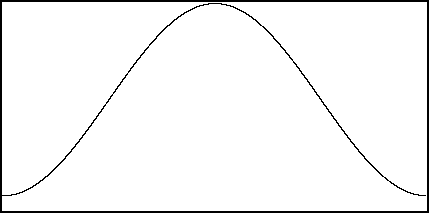
\includegraphics[scale=1]{image1} 


 Hamming Window Function.


 \textbf{Hanning. }



 \textbf{Example 2. Hanning window function statement}

\begin{lstlisting}
f82   0   8192   20   2   1
        
\end{lstlisting}


 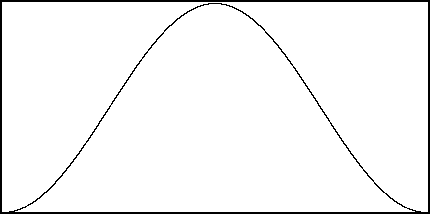
\includegraphics[scale=1]{image2} 


 Hanning Window Function


 \textbf{Bartlett. }



 \textbf{Example 3. Bartlett window function statement}

\begin{lstlisting}
f83   0   8192   20   3   1
        
\end{lstlisting}


 
\includegraphics[scale=1]{image3} 


 Bartlett Window Function


 \textbf{Blackman. }



 \textbf{Example 4. Blackman window function statement}

\begin{lstlisting}
f84   0   8192   20   4   1
        
\end{lstlisting}


 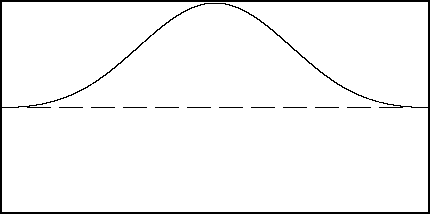
\includegraphics[scale=1]{image4} 


 Blackman Window Function


 \textbf{Blackman-Harris. }



 \textbf{Example 5. Blackman-Harris window function statement}

\begin{lstlisting}
f85   0   8192   20   5   1
        
\end{lstlisting}


 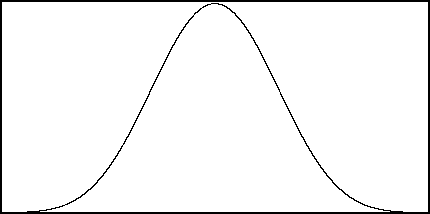
\includegraphics[scale=1]{image5} 


 Blackman-Harris Window Function


 \textbf{Gaussian. }



 \textbf{Example 6. Gaussian window function statement}

\begin{lstlisting}
f86   0   8192   20   6   1
        
\end{lstlisting}


 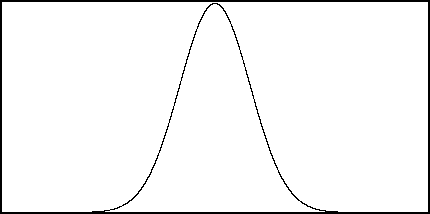
\includegraphics[scale=1]{image6} 


 Gaussian Window Function


 \textbf{Rectangle. }



 \textbf{Example 7. Rectangle window function statement}

\begin{lstlisting}
f88   0   8192   -20   8   .1
        
\end{lstlisting}
\emph{Note}
: Vertical scale is exaggerated in this diagram. 

 
\includegraphics[scale=1]{image7} 


 Rectangle Window Function


 \textbf{Sync. }



 \textbf{Example 8. Sync window function statement}

\begin{lstlisting}
f89   0   4096   -20   9   .75
        
\end{lstlisting}


 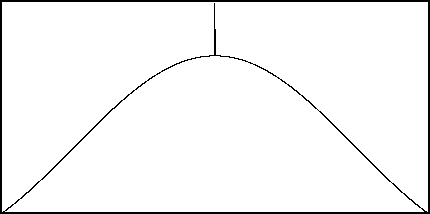
\includegraphics[scale=1]{image8} 


 Sync Window Function
%\hline 


\begin{comment}
\begin{tabular}{lcr}
Previous &Home &Next \\
Formant Values &� &SoundFont2 File Format

\end{tabular}


\end{document}
\end{comment}
